\documentclass[tikz, convert=pdf2svg]{standalone}

\usepackage{tikz}
\tikzset{>=stealth}
\usetikzlibrary{shapes,arrows}

% Define block styles
\tikzstyle{decision} = [diamond, draw, fill=blue!20, 
    text width=4.5em, text badly centered, node distance=3cm, inner sep=0pt]
\tikzstyle{block} = [rectangle, draw, fill=blue!20, 
    text centered, rounded corners, minimum height=2.5em]
\tikzstyle{input} = [rectangle, draw, fill=green!20, 
    text centered, rounded corners, minimum height=2.5em]
\tikzstyle{output} = [rectangle, draw, fill=green!60, 
    text centered, rounded corners, minimum height=2.5em]
\tikzstyle{line} = [draw, ->]
\tikzstyle{cloud} = [draw, ellipse,fill=red!20, node distance=3cm,
    minimum height=2em]

\usetikzlibrary{arrows.meta}
\tikzset{%
      >={Latex[width=2mm,length=2mm]},
}
\begin{document}
    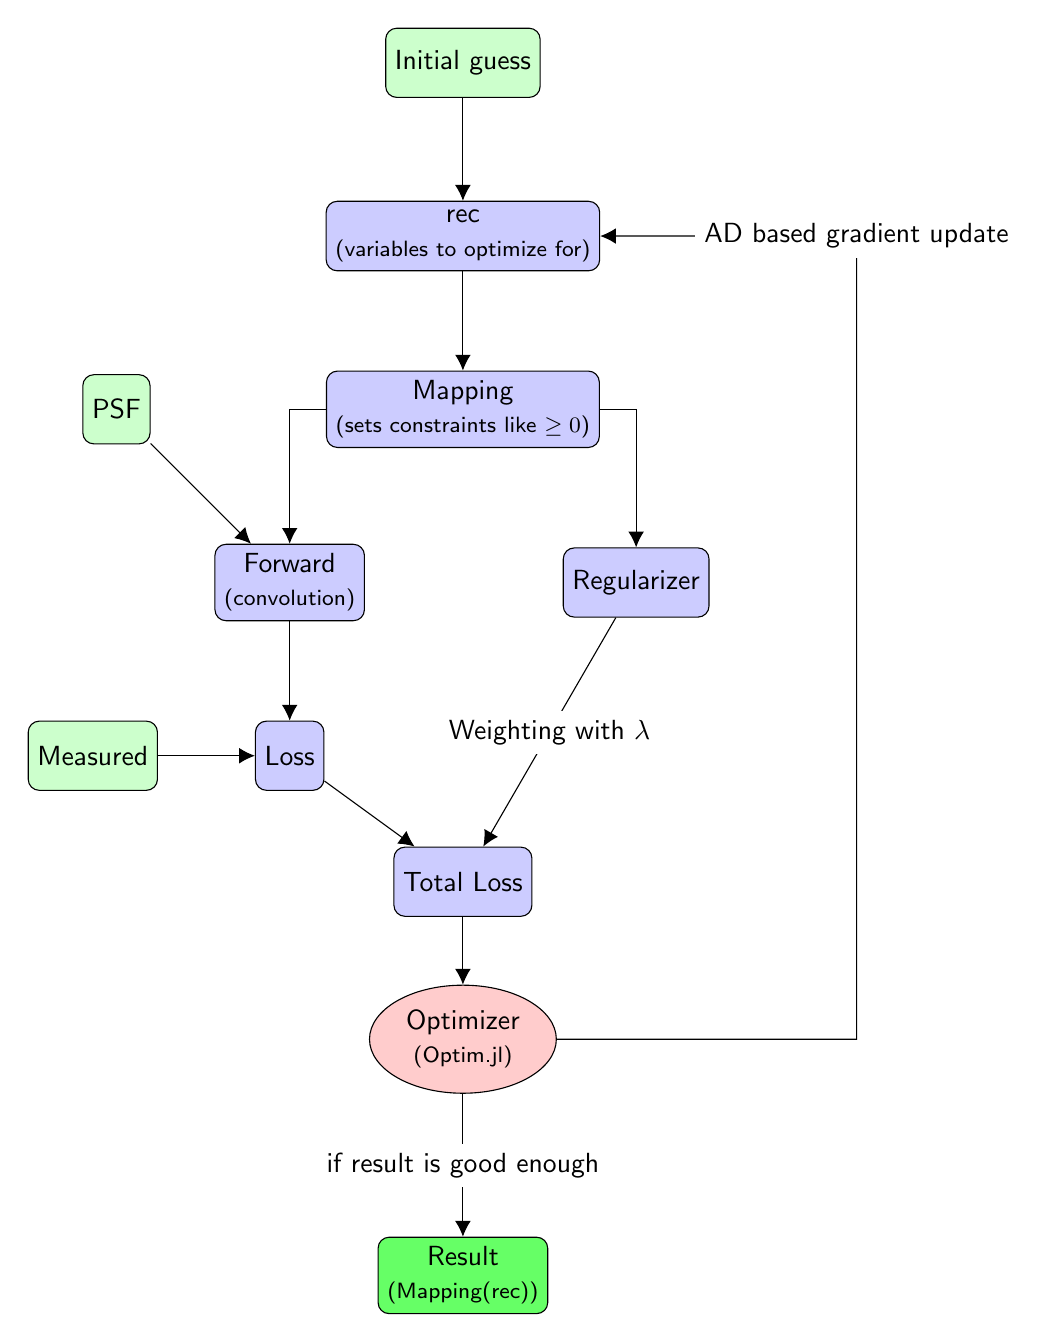
\begin{tikzpicture}[node distance=2.2cm,
    every node/.style={fill=white, font=\sffamily}, align=center]
        
        \node[block] (start) {rec \\\footnotesize (variables to optimize for)};
        \node[input, above of=start] (guess) {Initial guess};
        \node[block, below of=start] (map) {Mapping \\ \footnotesize (sets constraints like $\geq 0$)};
        \node[block, below of=map, left of=map] (forw) {Forward \\\footnotesize(convolution)};
        \node[block, below of=forw] (loss) {Loss};
        \node[block, below of=loss, right of=map] (reg) {Regularizer};
        
        \node[block, below of=map, node distance=6cm] (tloss) {Total Loss};
        \node[cloud, below of=tloss, node distance=2cm] (opt) {Optimizer\\\footnotesize (Optim.jl)};
   
        \node[input, left of=forw, above of=forw] (psf) {PSF}; 
        \node[input, left of=loss, node distance=2.5cm] (meas) {Measured}; 
    
        \node[output, node distance=3cm, below of=opt] (res) {Result \\ \footnotesize(Mapping(rec))};

        \path [line] (guess) -- (start);
        \path [line] (start) -- (map);
        \path [line] (map) -| (reg);
        \path [line] (map) -| (forw);
        \path [line] (forw) -- (loss);
        \path [line] (loss) -- (tloss);
        \path [line] (tloss) -- (opt);
        \path [line] (reg) --node [midway] {Weighting with $\lambda$} (tloss) ;
        \path [line] (opt) -- node[midway] {if result is good enough} (res);

            
        \path[line] (opt) --++ (5, 0) --++ (0, 10.2) node[] {AD based gradient update} -- (start) ;

        \path [line] (psf)-- (forw);
        \path [line] (meas)-- (loss);
    \end{tikzpicture}
\end{document}
